% !TEX root = ../../main.tex
\begin{figure*}[t]
  \centering
  % adjust margin to center captions
  \captionsetup[subfigure]{margin={0cm,0cm},oneside}
  \hspace*{\fill}%
  \begin{subfigure}[c]{0.5\linewidth}
    \centering
    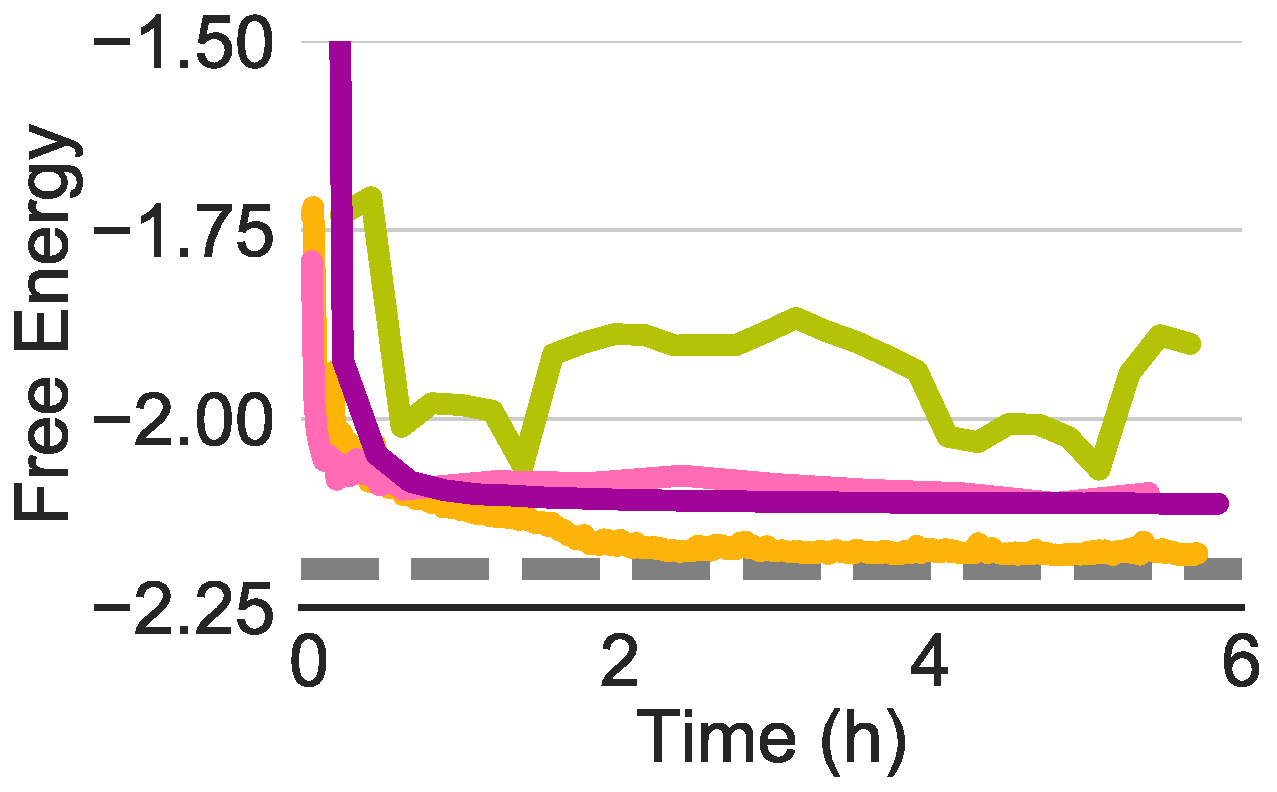
\includegraphics[width=\textwidth]{ch-hvm/fig/ising-large.pdf}
    % \caption{$\beta=0.4$}%
  \end{subfigure}
  % \hfill\hspace{\mywidth}%
  \begin{subfigure}[c]{0.3\linewidth}
    \centering
    % \raisebox{12mm}{
      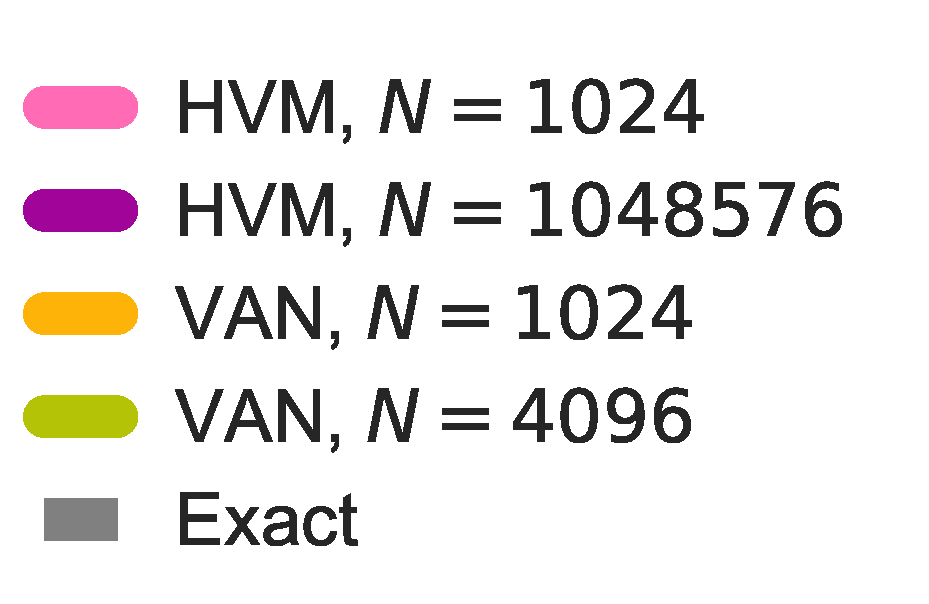
\includegraphics[width=\textwidth]{ch-hvm/fig/legend-ising}
    % }
  \end{subfigure}
  \hspace*{\fill}%
  % \vspace{-0.5cm}
  \caption[\textsc{hvm}s applied to the Ising model]{\textbf{\Acrfullpl{hvm} scale to statistical physics models with millions of random variables, with over 100x parameter savings.} The free energy is reported (the variational lower bound yields an upper bound on the free energy). The \gls{hvm} variational approximations use $5400$ parameters, while the \gls{van} method uses over $700$k.}
  \label{fig:hvm-ising}
\end{figure*}